%#!uplatex
%%%%%%%%%%%%%%%%%%%%%%%%%%%%%%%%%%%%%%%%%%%%%%%%%%%%%%%%%%%%%%%%%%%%%%%%%%%%%%%%%%%%%%%%%%%%%%%%%%%
%%%%%%%%%%%%%%%%%%%%%%%%%%%%%%%%%%%%%%%%%%%%%%%%%%%%%%%%%%%%%%%%%%%%%%%%%%%%%%%%%%%%%%%%%%%%%%%%%%%
%%%%%%%%%%%%%%%%%%%%%%%%%%%%%%%%%%%%%%%%%%%%%%%%%%%%%%%%%%%%%%%%%%%%%%%%%%%%%%%%%%%%%%%%%%%%%%%%%%%
\documentclass[12pt,dvipdfmx,uplatex]{beamer}
%%%%%%%%%%%%%%%%%%%%%%%%%%%%%%%%%%%%%%%%%%%%%%%%%%%%%%%%%%%%%%%%%%%%%%%%%%%%%%%%%%%%%%%%%%%%%%%%%%%
%%%%%%%%%%%%%%%%%%%%%%%%%%%%%%%%%%%%%%%%%%%%%%%%%%%%%%%%%%%%%%%%%%%%%%%%%%%%%%%%%%%%%%%%%%%%%%%%%%%
%%%%%%%%%%%%%%%%%%%%%%%%%%%%%%%%%%%%%%%%%%%%%%%%%%%%%%%%%%%%%%%%%%%%%%%%%%%%%%%%%%%%%%%%%%%%%%%%%%%
%%%
%%% hyperref 文字化け対策
%%%
\usepackage{pxjahyper}
\usepackage{hyperref}
%%%%%%%%%%%%%%%%%%%%%%%%%%%%%%%%%%%%%%%%%%%%%%%%%%%%%%%%%%%%%%%%%%%%%%%%%%%%%%%%%%%%%%%%%%%%%%%%%%%
%%%%%%%%%%%%%%%%%%%%%%%%%%%%%%%%%%%%%%%%%%%%%%%%%%%%%%%%%%%%%%%%%%%%%%%%%%%%%%%%%%%%%%%%%%%%%%%%%%%
%%%%%%%%%%%%%%%%%%%%%%%%%%%%%%%%%%%%%%%%%%%%%%%%%%%%%%%%%%%%%%%%%%%%%%%%%%%%%%%%%%%%%%%%%%%%%%%%%%%
%%%
%%% 各種パッケージ
%%%
\usepackage{graphicx}
%\usepackage{url,cite}
\usepackage{amsmath}
\usepackage{amsthm} \theoremstyle{definition} %theorem環境が斜体になるので注意
\usepackage{amssymb} % AMS-TeX
\usepackage{setspace}
\usepackage{multirow}
\usepackage{udline} % udline.sty

%%%%%%%%%%%%%%%%%%%%%%%%%%%%%%%%%%%%%%%%%%%%%%%%%%%%%%%%%%%%%%%%%%%%%%%%%%%%%%%%%%%%%%%%%%%%%%%%%%%
%%%%%%%%%%%%%%%%%%%%%%%%%%%%%%%%%%%%%%%%%%%%%%%%%%%%%%%%%%%%%%%%%%%%%%%%%%%%%%%%%%%%%%%%%%%%%%%%%%%
%%%%%%%%%%%%%%%%%%%%%%%%%%%%%%%%%%%%%%%%%%%%%%%%%%%%%%%%%%%%%%%%%%%%%%%%%%%%%%%%%%%%%%%%%%%%%%%%%%%
%%%
%%% 本文・数式フォント
%%%
\usepackage{newtxtext}
\usepackage[varg]{newtxmath}
%\usepackage{newpxtext}
%\usepackage[varg]{newpxmath}

% \mathcal(\cal)の扱い
%\DeclareMathAlphabet{\mathcal}{OMS}{cmsy}{m}{n} %computer modern
%\DeclareMathAlphabet{\mathcal}{OMS}{txsy}{m}{n} %txfont
%\usepackage[psamsfonts]{eucal} % euler

% mathptmx時に数式モードのvをtxfontから借りる
% \DeclareSymbolFont{lettersA}{U}{txmia}{m}{it}
% \SetSymbolFont{lettersA}{bold}{U}{txmia}{bx}{it}
% \DeclareFontSubstitution{U}{txmia}{m}{it}
% \DeclareMathSymbol{v}{\mathalpha}{lettersA}{"33} %"

%%%%%%%%%%%%%%%%%%%%%%%%%%%%%%%%%%%%%%%%%%%%%%%%%%%%%%%%%%%%%%%%%%%%%%%%%%%%%%%%%%%%%%%%%%%%%%%%%%%
%%%%%%%%%%%%%%%%%%%%%%%%%%%%%%%%%%%%%%%%%%%%%%%%%%%%%%%%%%%%%%%%%%%%%%%%%%%%%%%%%%%%%%%%%%%%%%%%%%%
%%%%%%%%%%%%%%%%%%%%%%%%%%%%%%%%%%%%%%%%%%%%%%%%%%%%%%%%%%%%%%%%%%%%%%%%%%%%%%%%%%%%%%%%%%%%%%%%%%%
%%%
%%%  日本語フォントをゴシックに、数式フォントを太字に変更する
%%%
\usepackage[deluxe]{otf}
\renewcommand{\kanjifamilydefault}{\gtdefault}
\renewcommand{\familydefault}{\sfdefault}

\setbeamerfont{title}{size=\large,series=\bfseries}
\setbeamerfont{frametitle}{size=\large,series=\bfseries}
%\setbeamertemplate{frametitle}[default][center]
\usefonttheme{professionalfonts} 

%%%
% Suppress Warning in the case of uplatex
\DeclareFontShape{JY2}{hgt}{b}{n}{<->ssub*hgt/bx/n}{}
\DeclareFontShape{JT2}{hgt}{b}{n}{<->ssub*hgt/bx/n}{}

%\mathversion{bold} %数式フォントを太字に

%%%%%%%%%%%%%%%%%%%%%%%%%%%%%%%%%%%%%%%%%%%%%%%%%%%%%%%%%%%%%%%%%%%%%%%%%%%%%%%%%%%%%%%%%%%%%%%%%%%%%%
%%% Beamer template preamble
%%%
%%% �ơ��ޤλ��ꡢ��ά���� default �ˤʤ�
%%%

 % �ե졼��λ��ꡢ��ά��
%%%%%%%%%%%%%%%%%%%%%%%%%%%% THEME
  %\usetheme{AnnArbor}
  %\usetheme{Antibes}
  %\usetheme{Bergen}
  %\usetheme{Berkeley}
  %\usetheme{Berlin}
  \usetheme{Boadilla}
  %\usetheme{boxes}
  %\usetheme{CambridgeUS}
  %\usetheme{Copenhagen}
  %\usetheme{Darmstadt}
  %\usetheme{default}
  %\usetheme{Dresden}
  %\usetheme{Frankfurt}
  %\usetheme{Goettingen}
  %\usetheme{Hannover}
  %\usetheme{Ilmenau}
  %\usetheme{JuanLesPins}
  %\usetheme{Luebeck}
  %\usetheme{Madrid}
  %\usetheme{Malmoe}
  %\usetheme{Marburg}
  %\usetheme{Montpellier}
  %\usetheme{PaloAlto}
  %\usetheme{Pittsburgh}
  %\usetheme{Rochester}
  %\usetheme{Singapore}
  %\usetheme{Szeged}
  %\usetheme{Warsaw}

% ����
%%%%%%%%%%%%%%%%%%%%%%%%%%%% COLOR THEME
  %\usecolortheme{albatross}
  %\usecolortheme{beetle}
  %\usecolortheme{crane}
  %\usecolortheme{default}
  %\usecolortheme{dolphin}
  %\usecolortheme{dove}
  %\usecolortheme{fly}
  %\usecolortheme{lily}
  %\usecolortheme{orchid}
  %\usecolortheme{rose}
  %\usecolortheme{seagull}
  %\usecolortheme{seahorse}
  %\usecolortheme{sidebartab}
  %\usecolortheme{structure}
  %\usecolortheme{whale}

% �إå����եå����ե졼��������ꡢ��ά��
  %%%%%%%%%%%%%%%%%%%%%%%%%%%% OUTER THEME
  %\useoutertheme{default}
  %\useoutertheme{infolines}
  %\useoutertheme{miniframes}
  %\useoutertheme{shadow}
  %\useoutertheme{sidebar}
  %\useoutertheme{smoothbars}
  %\useoutertheme{smoothtree}
  %\useoutertheme{split}
  %\useoutertheme{tree}

% �����ȥ롢section, itemize/enumerate �Ķ���
% theorem �Ķ�����, ����ʸ���ʤɤΥ����������ꡢ
% ����
  %%%%%%%%%%%%%%%%%%%%%%%%%%%% INNER THEME
  %\useinnertheme{circles}
  %\useinnertheme{default}
  %\useinnertheme{inmargin}
  \useinnertheme{rectangles}
  %\useinnertheme{rounded}


%\usefonttheme{}	% ����
%\logo{}		% ����
%\logo{\includegraphics[width=2cm]{titech_logo.eps}}

% navi. symbols����Ω���ʤ�����dvipdfmx��Ȥ��ȵ�ǽ���ʤ��Τ���ɽ����
\setbeamertemplate{navigation symbols}{}
%\setbeamertemplate{caption}[numbered]
%%%%%%%%%%%%%%%%%%%%%%%%%%%%%%%%%%%%%%%%%%%%%%%%%%%%%%%%%%%%%%%%%%%%%%%%%%%%%%%%%%%%%%%%%%%%%%%%%%%
%%%%%%%%%%%%%%%%%%%%%%%%%%%%%%%%%%%%%%%%%%%%%%%%%%%%%%%%%%%%%%%%%%%%%%%%%%%%%%%%%%%%%%%%%%%%%%%%%%%
%%%%%%%%%%%%%%%%%%%%%%%%%%%%%%%%%%%%%%%%%%%%%%%%%%%%%%%%%%%%%%%%%%%%%%%%%%%%%%%%%%%%%%%%%%%%%%%%%%%

% \AtBeginSection[] % Do nothing for \section*
% { \begin{frame}<beamer> \frametitle{}
%    \tableofcontents[currentsection,subsectionstyle=hide]
%  \end{frame} } 

%appendix��ڡ���������Ȥ��ʤ�
\newcommand{\backupbegin}{
   \newcounter{framenumberappendix}
   \setcounter{framenumberappendix}{\value{framenumber}}
}
\newcommand{\backupend}{
   \addtocounter{framenumberappendix}{-\value{framenumber}}
   \addtocounter{framenumber}{\value{framenumberappendix}} 
}
% �����Ķ�
% \newtheorem{theorem}{Theorem}
% \newtheorem{lemma}[theorem]{Lemma}
% \newtheorem{corollary}[theorem]{Corollary}
% \newtheorem{definition}[theorem]{Definition}
% \newtheorem{example}[theorem]{Example}
\newtheorem{proposition}{Proposition}
\newtheorem{remark}{Remark}


%%%%%%%%%%%%%%%%%%%%%%%%%%%%%%%%%%%%%%%%%%%%%%%%%%%%%%%%%%%%%%%%%%%%%%%%%%%%%%%%%%%%%%%%%%%%%%%%%%%%%%
% �Ƽ拾�ޥ�������
\def\Fig#1{Fig.\@\ref{#1}}
\def\Table#1{Table~\ref{#1}}
\def\Eq#1{Eq.\@(\ref{#1})}
\def\Eqs#1{Eqs.\@(\ref{#1})}
\def\Thm#1{Theorem~\ref{#1}}
\def\Lma#1{Lemma~\ref{#1}}
\def\Sect#1{Section~\ref{#1}}
\def\Rmk#1{Remark~\ref{#1}}
\def\Prop#1{Proposition~\ref{#1}}
\def\Coro#1{Corollary~\ref{#1}}
\def\Def#1{Definition~\@\ref{#1}}
\def\Prob#1{Problem~\@\ref{#1}}
\def\ie{{i.\@e.\@,~}}
\def\eg{{e.\@g.\@,~}}
\def\etal{{et al.}}

% �����Ķ���
\def\rank{\mathsf{rank}\, }
\def\dim{\mathsf{dim}\, }
\def\rspace{\mathsf{span}}
\def\supp{\mathsf{supp}}
%\def\vec#1{\mathbf{#1}}
\def\F{\mathbb{F}}
\def\wt{\mathsf{wt}}
\def\c{\mathcal{C}}
\def\dc{\mathcal{C}^{\perp}}
\def\d{\mathcal{D}}
\def\dd{\mathcal{D}^{\perp}}
\def\g{\mathcal{G}}
\def\dg{\mathcal{G}^{\perp}}
\def\p{\mathcal{P}}
% \def\rspace{\mathsf{span}}
\def\supp{\mathsf{supp}}
\def\ker{\mathsf{Ker\ }}

%\def\bari#1{\{\widebar{#1}\}}
\def\bari#1{\,\overline{{\!\{#1\}\!}}\,}
%\def\bari#1{\bar{\{#1\}}}
\def\vecxi{Z_{\bari{i}}}
%\def\vecsxi{\vec{z}_i}
\def\tvector{X}
\def\tpackets{X_1,\dots,X_n}
\def\mvector{S}
\def\mpackets{S_1,\dots,S_l}
\def\rvector{Y}
\def\wvector{W}
\def\cvector{C}
\def\cword{C_{1},\dots,C_{l+n}}
\def\pcword{C_{l+1},\dots,C_{l+n}}
\def\randvector{R}

\def\compmat{\Phi}

%\def\vec#1{\mbox{\boldmath $#1$}}

%%%%%%%%%%%%%%%%%%%%%%%%%%%%%%%%%%%%%%%%%%%%%%%%%%%%%%%%%%%%%%%%%%%%%%%%%%%%%%%%%%%%%%%%%%%%%%%%%%%%%%
%���� widebar, Widebar
\usepackage{accents}
\makeatletter
\def\widebar{\accentset{{\cc@style\underline{\mskip11mu}}}}
\makeatother


%%%
%%% 著者など
%%%
\title[Modern Authentication]{Modern Authentication}
\subtitle{FIDO2 Web Authentication (WebAuthn) を学ぶ}
\author[Jun Kurihara]{栗原 淳}
\institute[U-Hyogo/Zettant]{兵庫県立大学 大学院応用情報科学研究科 \\ 株式会社ゼタント}
\date[\today]{\today}

%%%%%%%%%%%%%%%%%%%%%%%%%%%%%%%%%%%%%%%%%%%%%%%%%%%%%%%%%%%%%%%%%%%%%%%%%%%%%%%%%%%%%%%%%%%%%%%%%%%
%%%%%%%%%%%%%%%%%%%%%%%%%%%%%%%%%%%%%%%%%%%%%%%%%%%%%%%%%%%%%%%%%%%%%%%%%%%%%%%%%%%%%%%%%%%%%%%%%%%
%%%%%%%%%%%%%%%%%%%%%%%%%%%%%%%%%%%%%%%%%%%%%%%%%%%%%%%%%%%%%%%%%%%%%%%%%%%%%%%%%%%%%%%%%%%%%%%%%%%
%%%%%%%%%%%%%%%%%%%%%%%%%%%%%%%%%%%%%%%%%%%%%%%%%%%%%%%%%%%%%%%%%%%%%%%%%%%%%%%%%%%%%%%%%%%%%%%%%%%
%%%%%%%%%%%%%%%%%%%%%%%%%%%%%%%%%%%%%%%%%%%%%%%%%%%%%%%%%%%%%%%%%%%%%%%%%%%%%%%%%%%%%%%%%%%%%%%%%%%

\begin{document}

\begin{frame}
\titlepage
\end{frame}

%%%%%%%%%%%%%%%%%%%%%%%%%%%%%%%%%%%%%%%%%%%%%%%%%%%%%%%%%%%%%%%%%%%%%%%%%%%%%%%%%%%%%%%%%%%%%%%%%%%
\section{はじめに}
\begin{frame}
 \centering
 {\Large はじめに}
\end{frame}

\begin{frame}{はじめに}
この講義では、
\begin{itemize}
 \item パスワード認証に代わるモダンな認証方式「FIDO」の概要
 \item FIDOの認証をWebブラウザ経由で利用する「FIDO2 WebAuthn」の利用
\end{itemize}
のさわりを学ぶ。
\end{frame}

\begin{frame}{この講義の対象と事前準備}
対象:
\begin{itemize}
\item 暗号・セキュリティ技術に興味がある初学者
\item Webに新しい認証技術を導入したいWeb系のエンジニア
\end{itemize}

\vspace{2ex}

※但し、ある程度の公開鍵暗号・電子署名の知識を前提とする\footnote[frame]{\scriptsize どういうものか、というのを知っていれば十分。「JavaScriptを使って学ぶEnd-to-Endセキュリティ」の資料を読んでいることを推奨 (\url{https://github.com/junkurihara/class-e2e_security_js})。}

\vspace{2ex}

必須ではないが触って楽しむのには必要な事前準備:
\begin{itemize}
\item Bash/Zsh, Gitが使えるようになっていること
\item Node.js, npm, yarnが使えるようになっていること
\item Google Chrome系ブラウザ and/or Firefoxが利用可能なこと
\end{itemize}
\end{frame}



%%%%%%%%%%%%%%%%%%%%%%%%%%%%%%%%%%%%%%%%%%%%%%%%%%%%%%%%%%%%%%%%%%%%%%%%%%%%%%%%%%%%%%%%%%%%%%%%%%%
\section{パスワード認証からFIDOへ}
\begin{frame}
\centering
{\Large パスワード認証からFIDOへ}
\end{frame}

\begin{frame}{認証とは}
\begin{block}{認証}
 「何らかの手段」で\alert{対象の正当性を確認する}こと。
\end{block}
\begin{itemize}
 \item メッセージの正当性を確認 $\Rightarrow$ メッセージ認証
 \item サービス利用ユーザの正当性を確認 $\Rightarrow$ ユーザ認証
 \item etc.
\end{itemize}

\vspace{2ex}

※このスライドで単純に「認証」と呼んだときは、\ul{認証対象を「正規ユーザ本人」としたユーザ認証・本人認証を指す}こととする。
\end{frame}

\begin{frame}{本人認証の3つの要素}
本人認証において、正当性確認のため検証されるものは大きく3要素に分類。
\begin{itemize}
 \item \textbf{知識}\\
$\Rightarrow$ 本人しか知らない知識を持っていればOK (ex. パスワード)
 \item \textbf{所有物}\\
$\Rightarrow$ 本人しか持っていない物を提示できればOK (ex. HWキー)
 \item \textbf{生体}\\
$\Rightarrow$ 本人の体の一部を提示できればOK (ex. 指紋)
\end{itemize}
\begin{center}
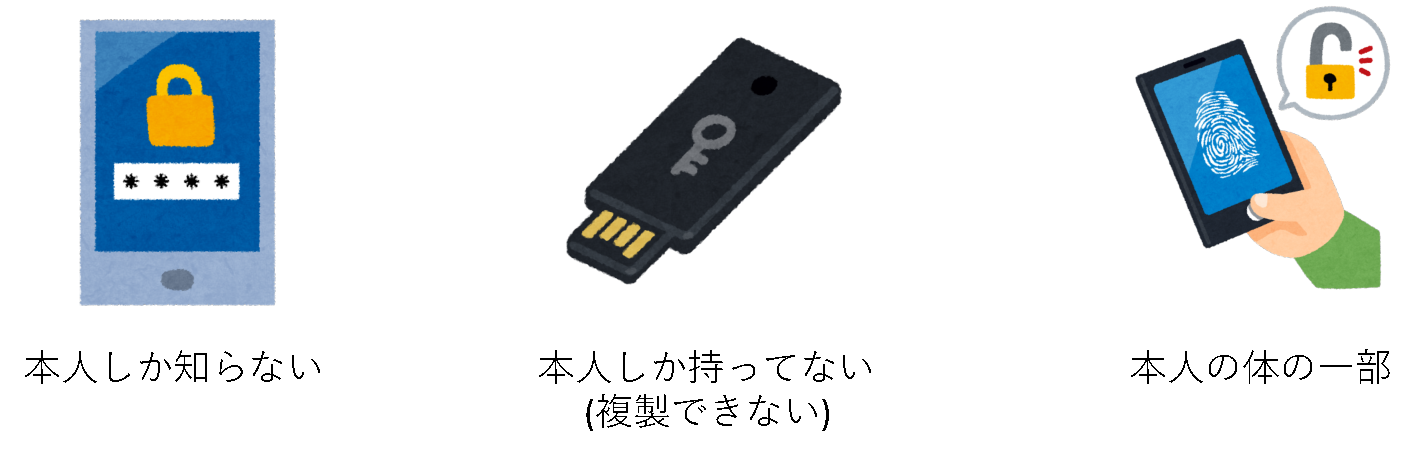
\includegraphics[width=0.7\linewidth]{Figs/auth-three-elements.pdf}
\end{center}

\end{frame}

\begin{frame}{オンラインサービスでのパスワード認証}
\begin{itemize}
\item サービスの利用者の識別子 (ID) と対応するパスワードをサービス事業者に登録、サービス利用時に利用者が自分のIDとパスワードを入力する。
\item パスワードは個人の記憶にのみ存在するため、\alert{パスワードを知っている人はそのサービスに登録してる本人と同一人物}と考えることができる。
\end{itemize}

\begin{center}
おそらく、誰にとっても最も馴染み深い認証方式! 
\end{center}

\end{frame}

\begin{frame}
\begin{figure}
\centering
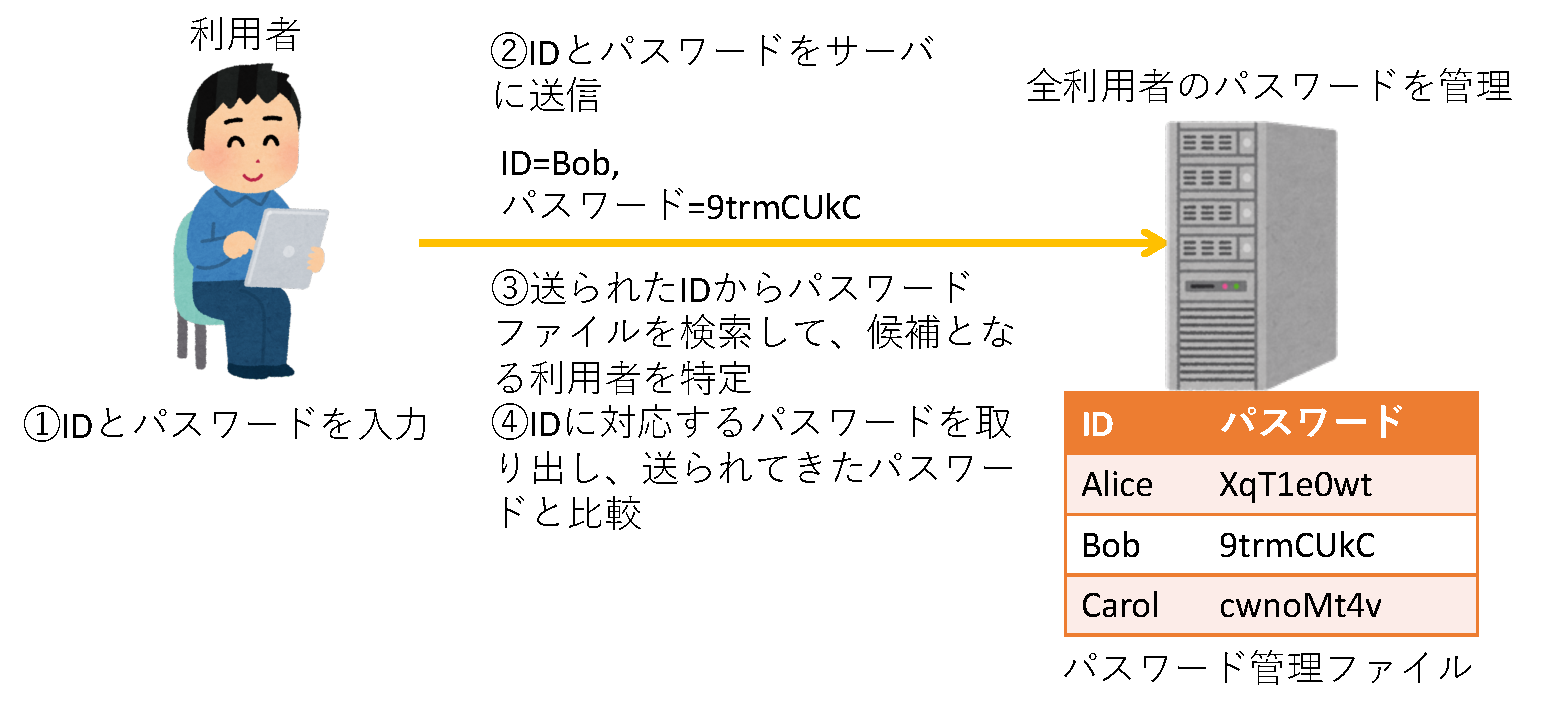
\includegraphics[width=\linewidth]{Figs/password-auth.pdf}\\
\caption{オンラインでの単純なパスワード認証}
\end{figure}
\end{frame}


\begin{frame}{オンラインでのパスワード認証の問題}
英数字・記号を組み合わせたパスワード:
\begin{itemize}
 \item 攻撃者にとって比較的\textbf{予測しやすい}\footnote[frame]{\scriptsize しかもオンラインだと予測→認証トライを繰り返せる}
 \item 「強い」パスワードを使わせるには\textbf{ユーザ教育が必要}\footnote[frame]{\scriptsize 教育なしだと覚え易く「弱い」ものを利用しがち}
 \item \textbf{覚えられない}
 \item etc...
\end{itemize}

\vspace{-5ex}
\begin{center}
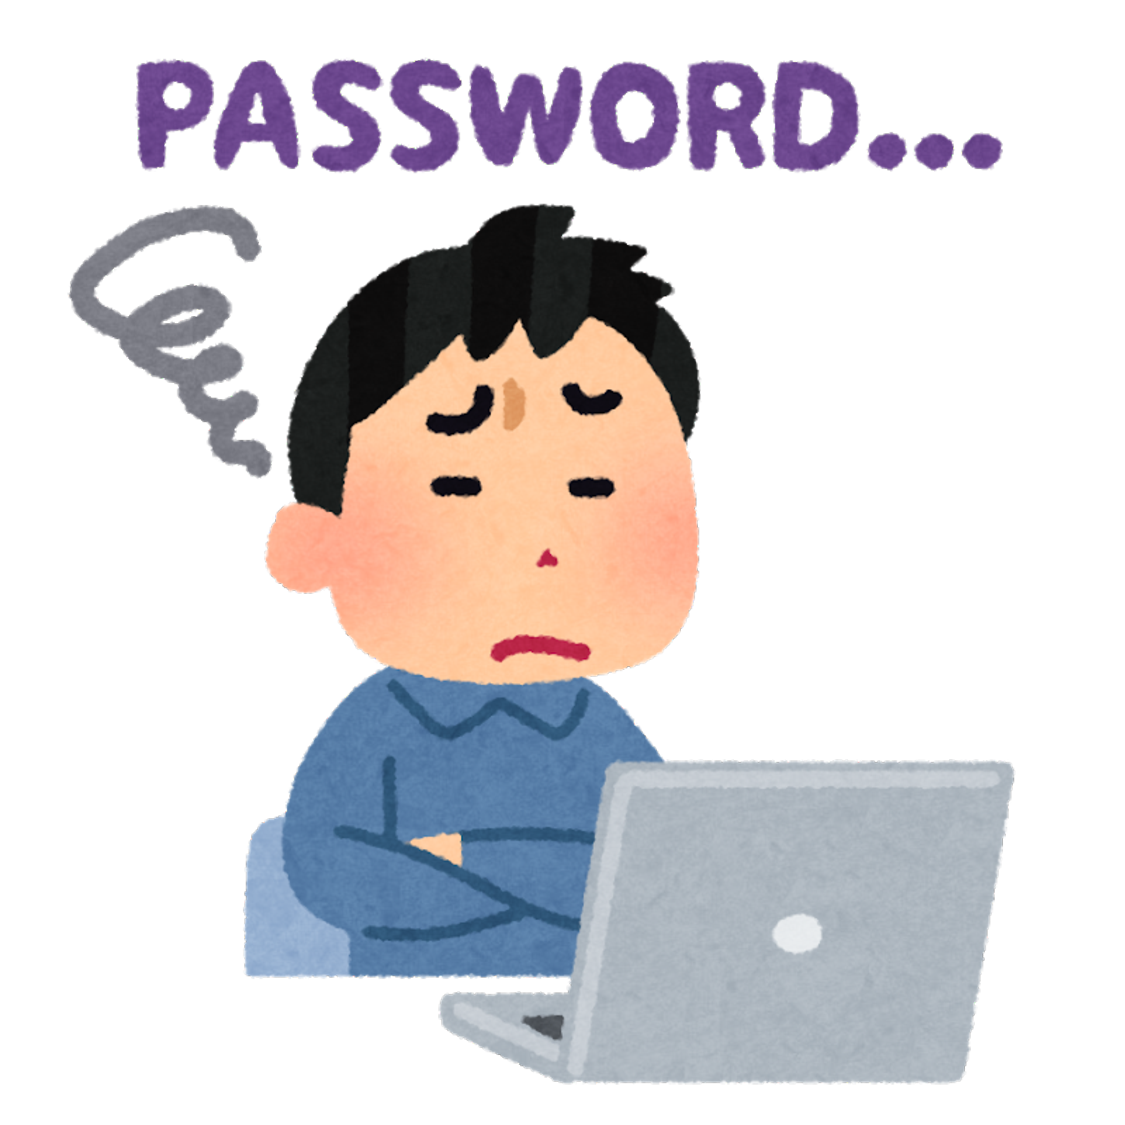
\includegraphics[width=0.2\linewidth]{Figs/password-forget.pdf}
\end{center}
\vspace{-2ex}

\structure{予測できず、誰が使っても強力で、確実に認証できる方法}が必要\\
$\Rightarrow$ \alert{ハードウェアセキュリティキーを使った認証}が人気に\\
$\Rightarrow$ \textbf{FIDOはそのような手法の\ul{標準化された方式}}

\end{frame}

\begin{frame}{FIDO}

\begin{block}{\small FIDO (Fast IDentity Online)}
業界団体FIDO Alliance\footnote[frame]{\scriptsize \url{https://fidoalliance.org}}の策定する、\alert{ハードウェアセキュリティキー+生体認証\footnote[frame]{\scriptsize すなわち、「所有物」と「生体」の二要素を同時に使った認証が可能。}と公開鍵暗号方式をベースとしたオンラインでの本人認証技術}。
\end{block}

現在はFIDO2 (v2.0) が最新の規格。以降、FIDO2の内容について触れていく。

\vspace{2ex}

厳密には、\structure{FIDO2はパスワードレス認証をサポートしつつも、パスワード+デバイス・生体認証の多要素での認証もサポートする}。

\end{frame}

\begin{frame}{FIDO認証概略}
FIDO認証の特徴:
\begin{itemize}
 \item 公開鍵暗号を利用した、オンラインでの認証方式の提供
 \item 認証器によるローカルでの本人認証
 \item 認証器内部に閉じた署名生成\\ $\Rightarrow$\alert{秘密鍵・パスワード等の秘密情報は外部に出ない}
\end{itemize}
\begin{figure}
\begin{center}
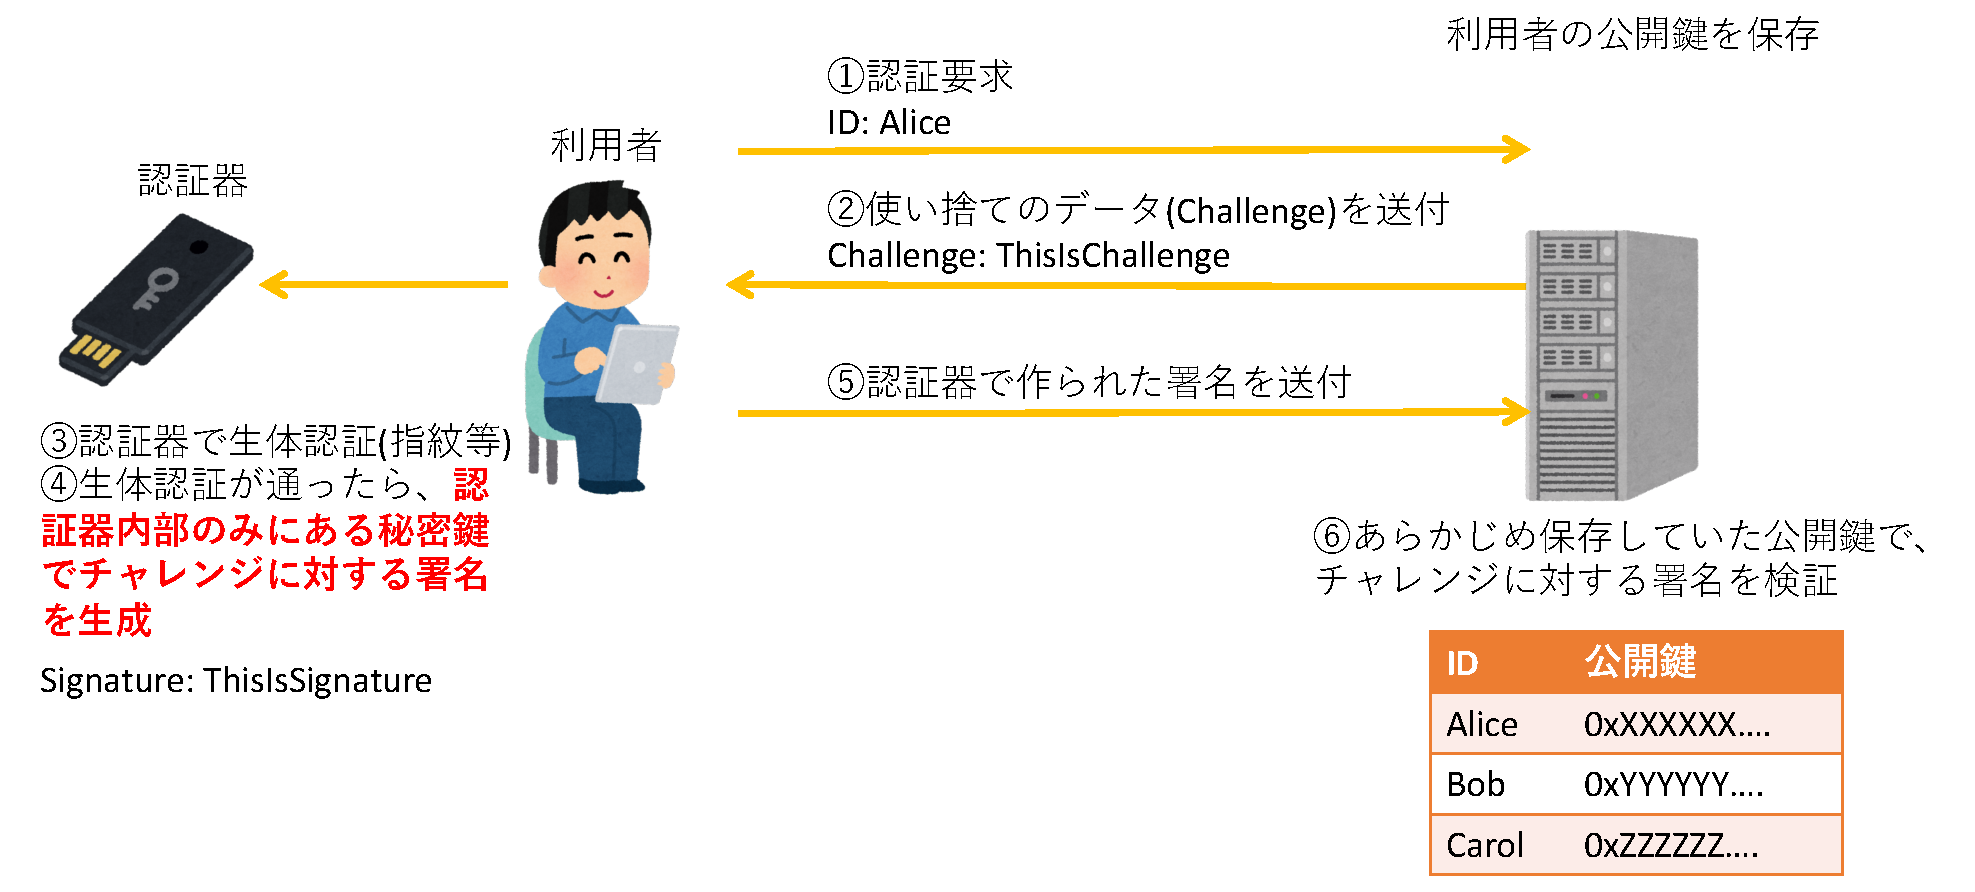
\includegraphics[width=0.9\linewidth]{Figs/FIDO2-auth.pdf}
\caption{FIDO認証概略}
\end{center}
\end{figure}
\end{frame}

\begin{frame}{FIDO2の要素}
FIDO2は、\alert{WebAuthn (Web Authentication)\footnote[frame]{\tiny Spec: \url{https://www.w3.org/TR/webauthn-1/}}と、CTAP (Client-to-Authenticator Protocol)\footnote[frame]{\tiny Spec: \url{https://fidoalliance.org/specs/fido2/fido-client-to-authenticator-protocol-v2.1-rd-20191217.html}}の2つの要素で構成}される。

\begin{figure}
\begin{center}
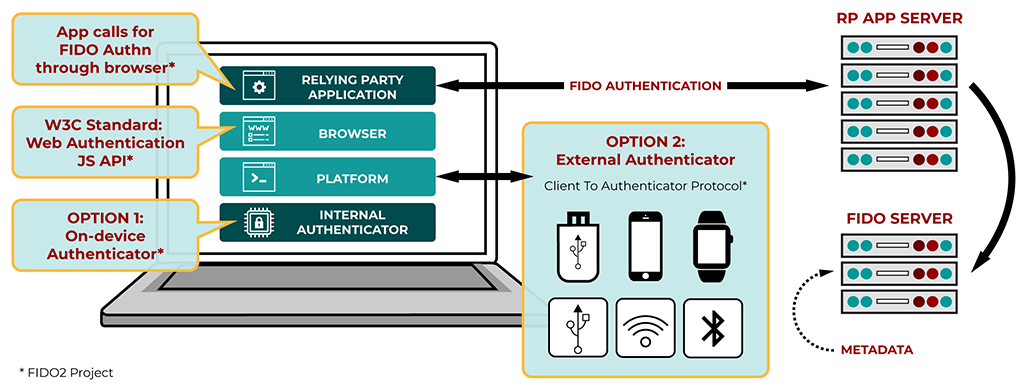
\includegraphics[width=0.9\linewidth]{Figs/FIDO2-Graphic-v2.png}
\caption{\footnotesize \textcopyright FIDO Alliance, from \url{https://fidoalliance.org/specifications/}}
\end{center}
\end{figure}
\end{frame}

\begin{frame}
\small 
\begin{itemize}
 \item \textbf{WebAuthn}: 内部/外部認証器をCallするWebAPIと、WebApp・サーバ間のデータフローを規定。
 \item \textbf{CTAP}: 外部認証器をCallするAPIと、クライアント/プラットフォームと認証器の通信プロトコルを規定。
\end{itemize}
\begin{center}
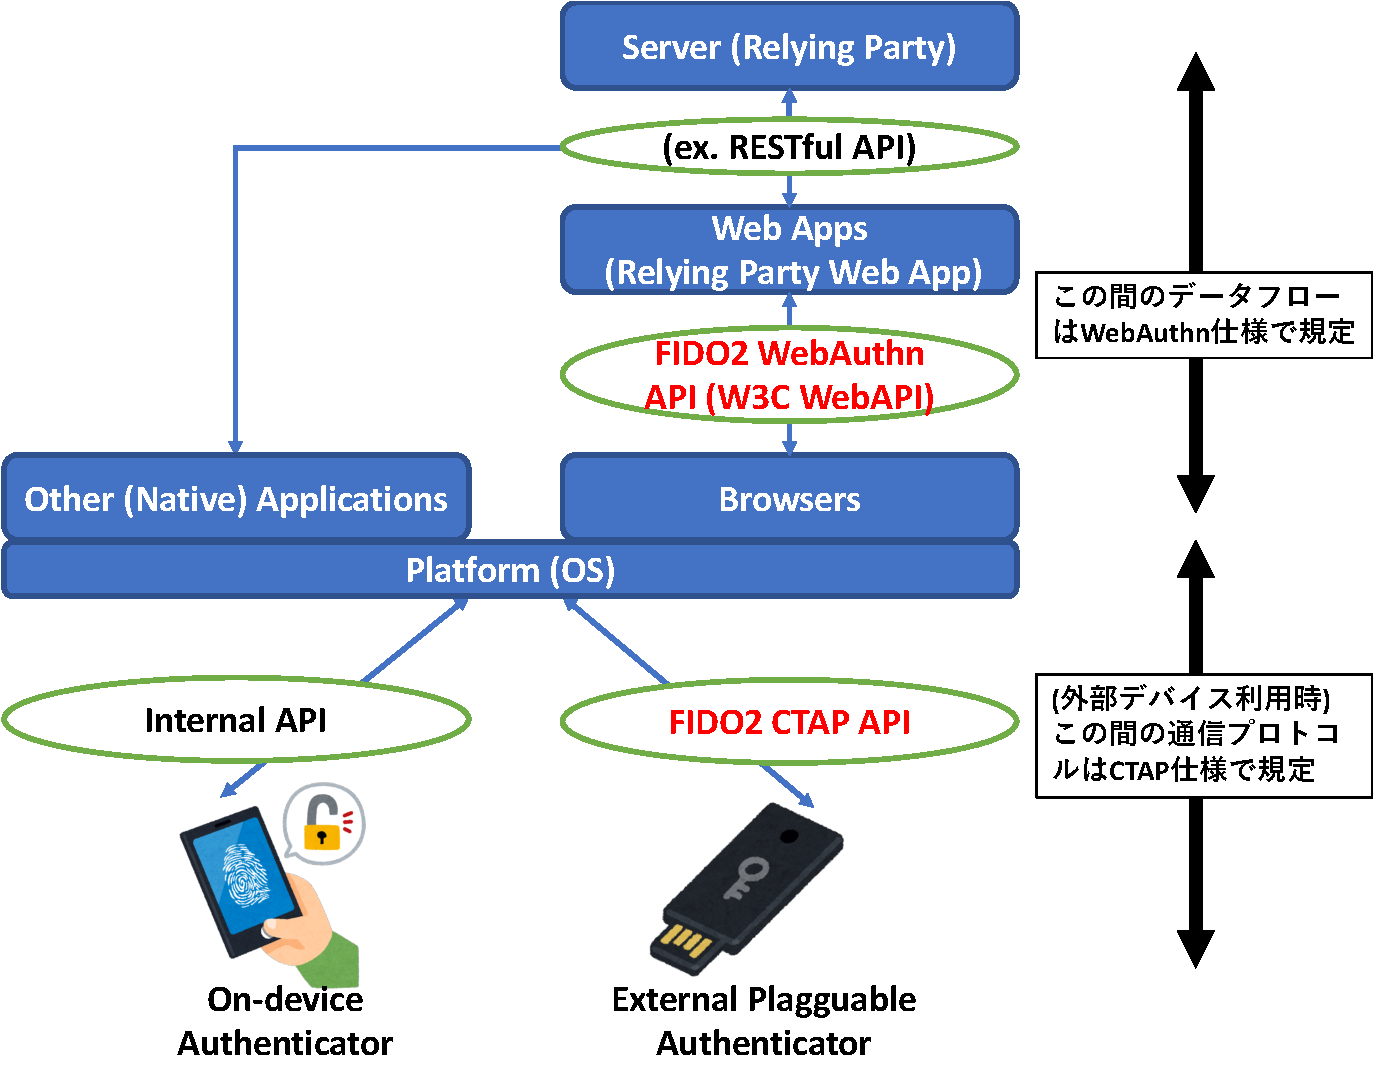
\includegraphics[width=0.7\linewidth]{Figs/FIDO2-spec-structure.pdf}
\end{center}
\end{frame}

\begin{frame}
\begin{block}{\small FIDO2 CTAP\footnote[frame]{\tiny \url{https://fidoalliance.org/specs/fido-v2.0-ps-20190130/fido-client-to-authenticator-protocol-v2.0-ps-20190130.html}}}
USB/BLE/NFC等で接続されたHWセキュリティキーなどの\alert{外部認証器と、クライアントアプリ(ブラウザ等)およびプラットフォーム(OS)との間の通信プロトコル}を規定。以下の要素で構成。
\begin{itemize}
\item USB/BLE/NFCなど物理層の種別に応じた、通信確立のためのプロトコル
\item 認証器での処理をCallするAPI
\begin{itemize}
\item 外部認証器の情報取得
\item PINによるローカルでのユーザ認証\footnote[frame]{\tiny 指紋認証やジェスチャーなどは認証器のみで完結するのでAPIは用意されない。署名生成などのときに認証器内での認証を要求するフラグを立てる。}
\item 認証器組込の秘密鍵での、ユーザ秘密鍵・証明書生成
\item ユーザ秘密鍵による署名の生成、など
\end{itemize}
\end{itemize}
\end{block}
ブラウザ・OS(のドライバ)は上記を実装した上で、より上位のWebAuthnのプロトコルをサポート。
\end{frame}


\begin{frame}
\begin{block}{\small FIDO2 WebAuthn\footnote[frame]{\tiny https://www.w3.org/TR/webauthn-1/}}
\alert{Webブラウザをプラットフォームとし、内部/外部認証器によって生成される署名を用いた、オンラインサーバでのユーザ認証のプロトコル}を規定。
より具体的には、以下を規定する。
\begin{itemize}
 \item 認証器でのユーザの公開鍵証明書の生成、サーバへの登録プロトコル
 \item 認証器での署名生成、サーバでの認証プロトコル
 \item 認証器とやりとりするためブラウザが具備すべきWeb API\footnote[frame]{\tiny JavaScriptでCallされるAPI。ブラウザの内部でさらに認証器のAPI (CTAPや内部API) をCallする。}。大雑把に以下の2種類。
\begin{itemize}
 \item ユーザの公開鍵証明書の生成 (Credential Creation)
 \item ユーザ秘密鍵による署名の生成 (Assertion Generation)
\end{itemize}
\end{itemize}
\end{block}
認証器とのやり取りはブラウザ/プラットフォームがサポート。\\
$\Rightarrow$ 基本的にWeb Appの観点からは、WebAuthnのみを意識する。
\end{frame}


\begin{frame}
\begin{exampleblock}{\small 補足: FIDO1}
\small
FIDO1 (v1.x) は、以下の2つの要素で構成されている。
\begin{itemize}
 \item UAF (Universal Authentication Framework): 生体認証機能を持つFIDO対応端末 (スマートフォン等) で\structure{パスワードレス認証}を行う機構。USB接続などの外部HWセキュリティキーは利用できない。
 \item U2F (Universal 2nd Factor)\footnote[frame]{\scriptsize U2FはFIDO2規格ではCTAP1と改称。FIDO2で追加された仕様はCTAP2と呼ばれる。}: ID・パスワード認証に加えた\structure{2要素認証}を行うのに、外部HWセキュリティキーを利用可能とする機構。
\end{itemize}
FIDO2は、UAFとU2Fを統合し、さらに外部HWキーを用いてもパスワードレス認証可能な、より利便性の高い規格と見做せる。
\end{exampleblock}
 
\end{frame}


\begin{frame}
\frametitle{FIDO2対応の認証器}
USB/NFC/BLE等対応の外部認証器 (External Authenticator)、端末付属の認証器 (On-device/Internal Authenticator) 共々、様々な対応デバイスがリリースされつつある。
\begin{tabular}{ccc}
\begin{minipage}[t]{0.3\linewidth}
\footnotesize
\centering
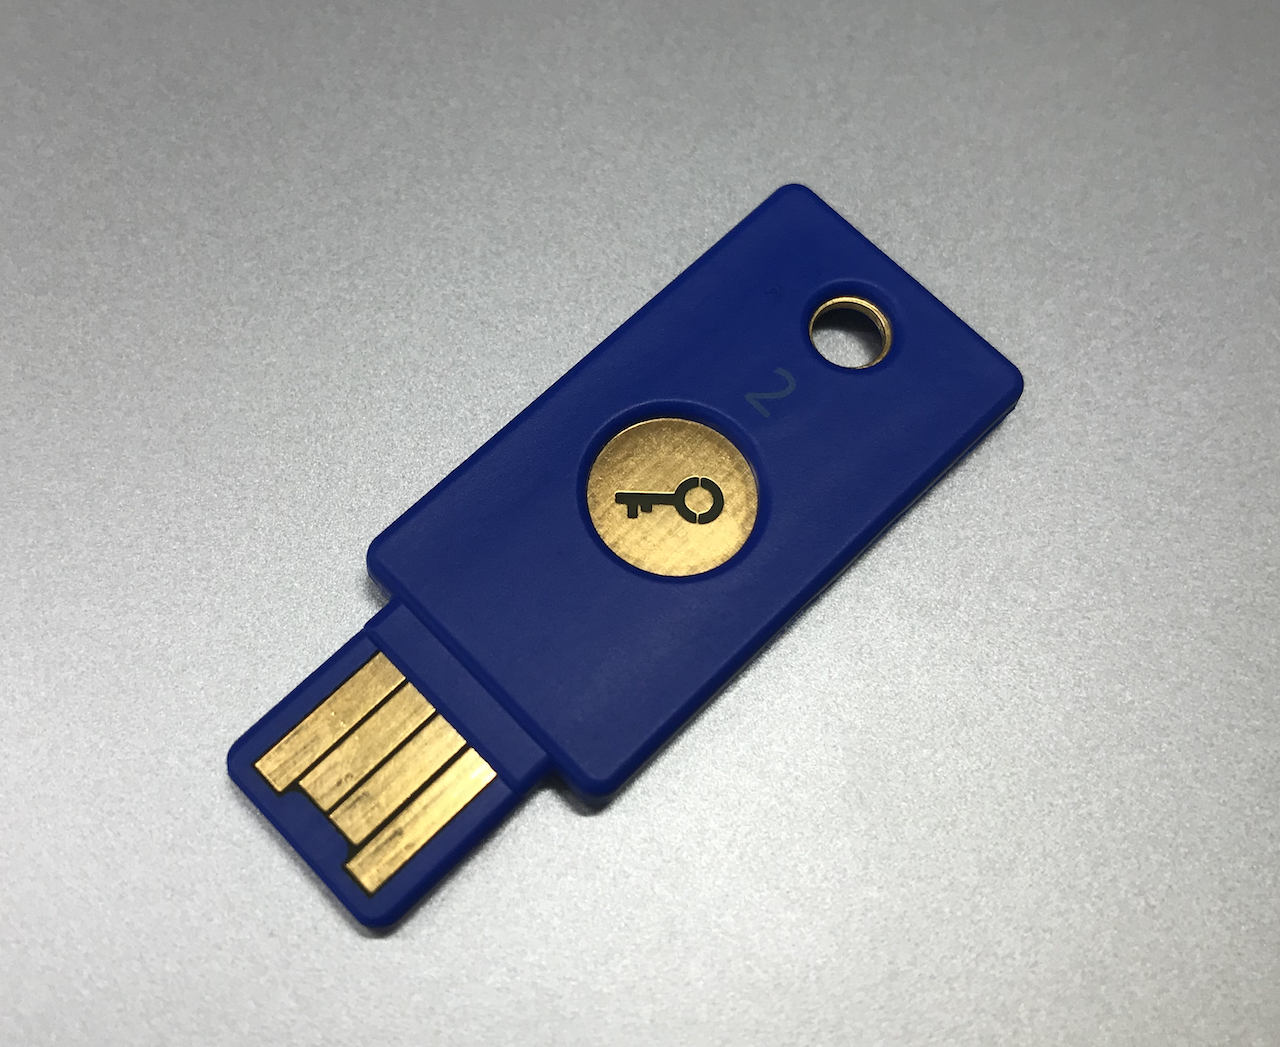
\includegraphics[width=\linewidth]{Figs/security-key-by-yubico.png}\\
\textbf{Security Key by Yubico}\\
FIDO2専用\footnote[frame]{\scriptsize FIDO2 CTAP1=FIDO1 U2Fには対応。}
\end{minipage}
& 
\begin{minipage}[t]{0.3\linewidth}
\footnotesize
\centering
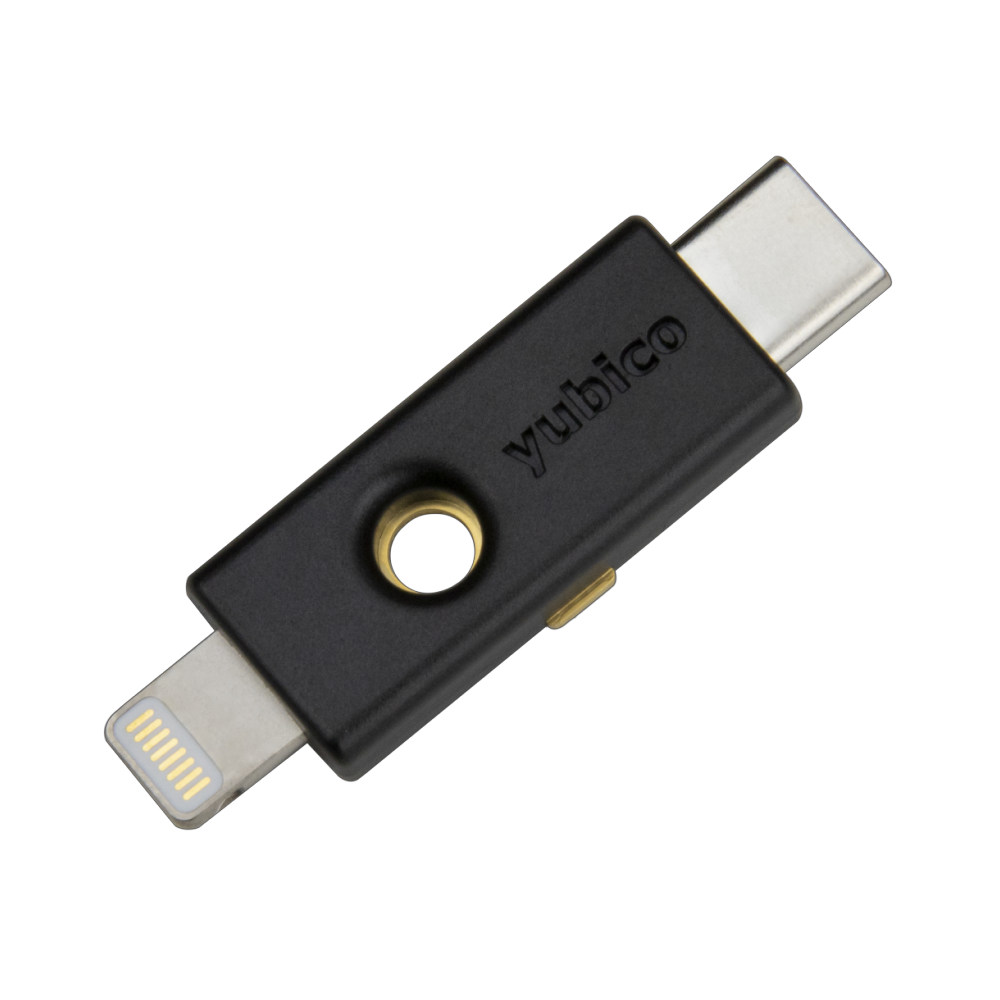
\includegraphics[width=\linewidth]{Figs/yubikey-5ci.png}\\
\textbf{YubiKey 5Ci}\\
FIDO2+OpenPGP+etc...
\end{minipage}
&
\begin{minipage}[t]{0.3\linewidth}
\footnotesize
\centering
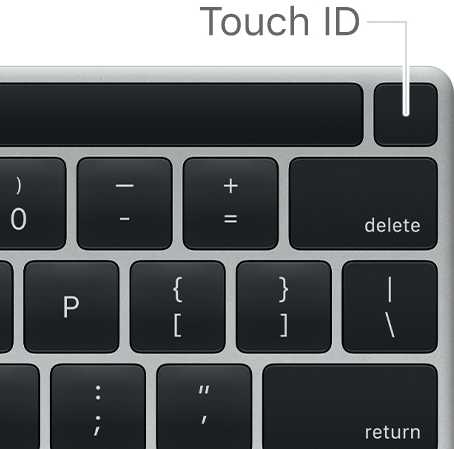
\includegraphics[width=\linewidth]{Figs/macbookpro-touchid.png}\\
\textbf{MacbookPro TouchID}\\
FIDO2認証可能\footnote[frame]{\scriptsize ブラウザ等がTouchID APIをCallできればFIDO2のOn-device Authenticatorとして動作。Chrome等は対応済。}
\end{minipage}
\end{tabular}
\end{frame}


\begin{frame}{FIDO2標準化状況}

FIDOは業界団体の策定した規格ではあるが、

\begin{itemize}
 \item \textbf{FIDO2 CTAP}: ITU-Tで勧告として国際標準化\footnote[frame]{\scriptsize \url{https://fidoalliance.org/fido-alliance-specifications-now-adopted-as-itu-international-standards/}}
 \item \textbf{FIDO2 WebAuthn}: W3Cで勧告として国際標準化\footnote[frame]{\scriptsize \url{https://www.w3.org/2019/03/pressrelease-webauthn-rec.html.ja}}
\end{itemize}

と、認証器とプラットフォーム/ブラウザ間の通信プロトコル、サーバ・ブラウザ間の認証プロトコルの両者共に国際標準として策定済。

\end{frame}

\begin{frame}
この後、FIDO2 WebAuthnの内容に実際に触れ、最新の認証技術について理解を深めてみよう。\footnote[frame]{\scriptsize 今回はWeb技術から学ぶセキュリティに注力するため、ローレイヤのFIDO2 CTAPについては別の機会で。}
\end{frame}

%%%%%%%%%%%%%%%%%%%%%%%%%%%%%%%%%%%%%%%%%%%%%%%%%%%%%%%%%%%%%%%%%%%%%%%%%%%%%%%%%%%%%%%%%%%%%%%%%%%
\section{サンプルコードの準備}
\begin{frame}
\centering
{\Large サンプルコードの準備}
\end{frame}

\begin{frame}{準備}
説明を聞きつつ手を動かすため、まず環境準備。

\vspace{2ex}

今回は以下の2つをWebAuthnのAPIをCallしながら試す。
\begin{itemize}
\item 認証器を使ってユーザの公開鍵証明書を生成\\
$\Rightarrow$ 認証器からのメッセージを解してみて\structure{実際に証明書および生の公開鍵を取り出してみる}。
\item 認証器を使ってユーザ認証用の証明を生成\\
$\Rightarrow$ 署名を解してみて、登録時に取り出した公開鍵で\structure{署名が通ることを確認してみる}。
\end{itemize}
$\Rightarrow$ この2つが\alert{FIDO2 WebAuthnのパスワードレス認証の基礎}。
\end{frame}

\begin{frame}
\frametitle{環境}

以下の環境が前提:
\begin{itemize}
 \item Node.js LTS ($\ge$ 12)がインストール済でyarnが使える\footnote[frame]{インストールコマンド: \texttt{npm i -g yarn}}
 \item ブラウザとして、Google Chrome (系ブラウザ)、もしくはFirefoxがインストール済み
 \item Visual Studio Code や WebStorm などの統合開発環境がセットアップ済みだとなお良い
\end{itemize}
\end{frame}

\begin{frame}
\frametitle{JavaScriptプロジェクトの準備}
\begin{enumerate}
\item \alert{プロジェクトのGitHubリポジトリをClone}\\
\begin{exampleblock}{}
\footnotesize
\$ \texttt{git clone https://github.com/junkurihara/xxxxxxxxxxxxxxxxxxxx}\\
\$ \texttt{cd sample}
\end{exampleblock}
\item 依存パッケージのインストール
\begin{exampleblock}{}
\$ \texttt{yarn install}
\end{exampleblock}
\item ライブラリのビルド
\begin{exampleblock}{}
\$ \texttt{yarn build}
\end{exampleblock}
\end{enumerate}
\end{frame}


%%%%%%%%%%%%%%%%%%%%%%%%%%%%%%%%%%%%%%%%%%%%%%%%%%%%%%%%%%%%%%%%%%%%%%%%%%%%%%%%%%%%%%%%%%%%%%%%%%%
\section{FIDO2 WebAuthnのフロー}
\begin{frame}
\centering
{\Large FIDO2 WebAuthnのフロー}
\end{frame}

\begin{frame}{FIDO2 WebAuthnのフローの参加エンティティ}
WebAuthnの動作フローでは、以下の3つの(抽象化された)参加エンティティが存在。
\begin{enumerate}
 \item \textbf{Relaying Party (RP)}: サービス提供者の認証サーバ
 \item \textbf{ブラウザ+RPのWebApp}: ユーザおよび認証器とやり取り
 \item \textbf{Authenticator}: 内部/外部認証器。以下をセキュアに保持。
\begin{itemize}
\item \textbf{\alert{Attestation Key Pair}}: 公開鍵・秘密鍵ペア
\item \textbf{\alert{Attestation Certificate}}: 上記の公開鍵に対し、FIDO2で承認された製造元が署名した証明書
\end{itemize}
\end{enumerate}
\end{frame}
\begin{frame}
\begin{center}
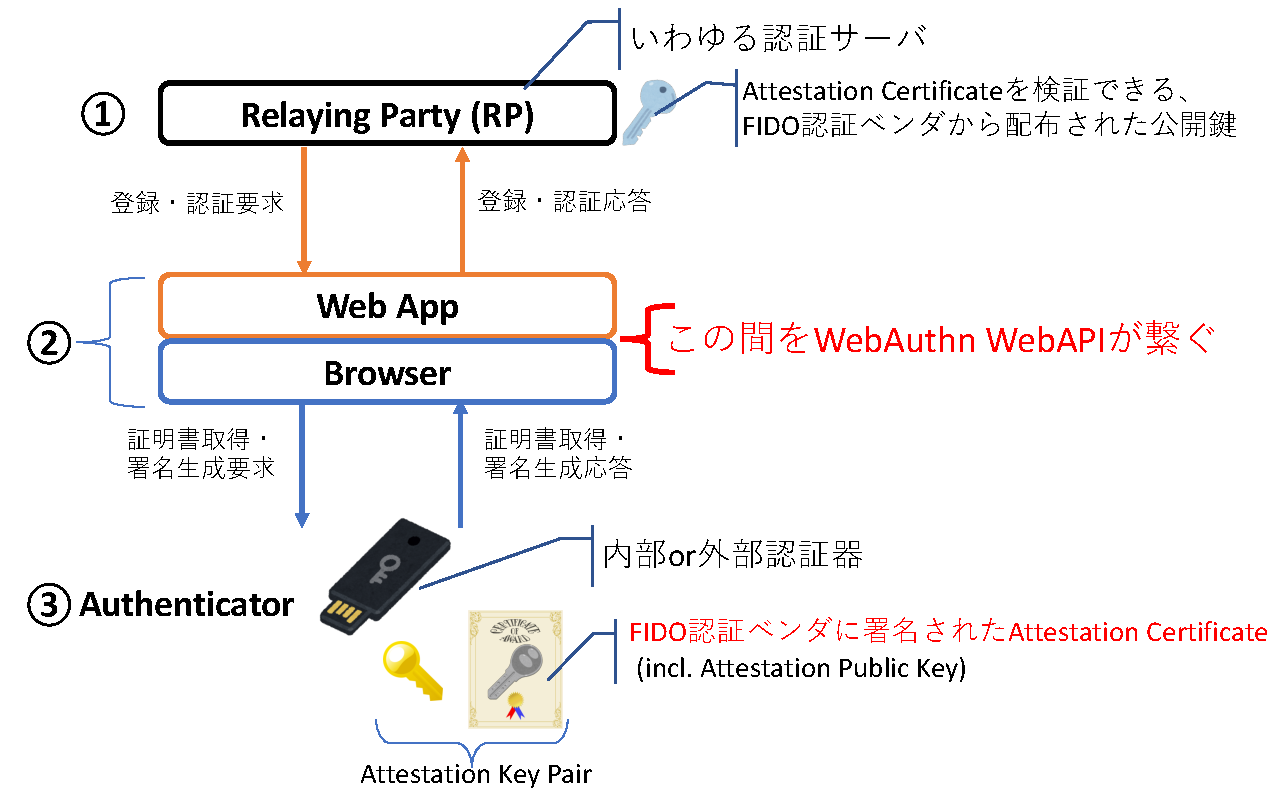
\includegraphics[width=0.9\linewidth]{Figs/webauthn-entities.pdf}
\end{center}
WebAPIとして用意されるWebAuthn APIは、ブラウザ経由でWebAppが認証器とやりとりする役割を担う。
\end{frame}

\begin{frame}{FIDO2におけるAttestation}
FIDO2では、「Attestation」という重要な概念が存在する。

\begin{block}{\small FIDO2におけるAttestation}
主として、「新しく生成・登録するユーザの公開鍵が、\alert{正しくFIDO2認定を受けている認証器で生成された公開鍵であることを保証する機構}という意味。すなわち、\textbf{出生証明}。
\end{block}
\begin{center}
\begin{tabular}{ll}
\begin{minipage}[c]{0.8\linewidth}
Relaying Partyは、出生証明を確認してユーザを登録。\\
$\Rightarrow$ 偽造認証器を摑まされたユーザの登録を弾ける。\\
$\Rightarrow$ \textbf{認証器に基づくFIDO2認証の安全性は維持}。
\end{minipage}
 &
\begin{minipage}[c]{0.15\linewidth}
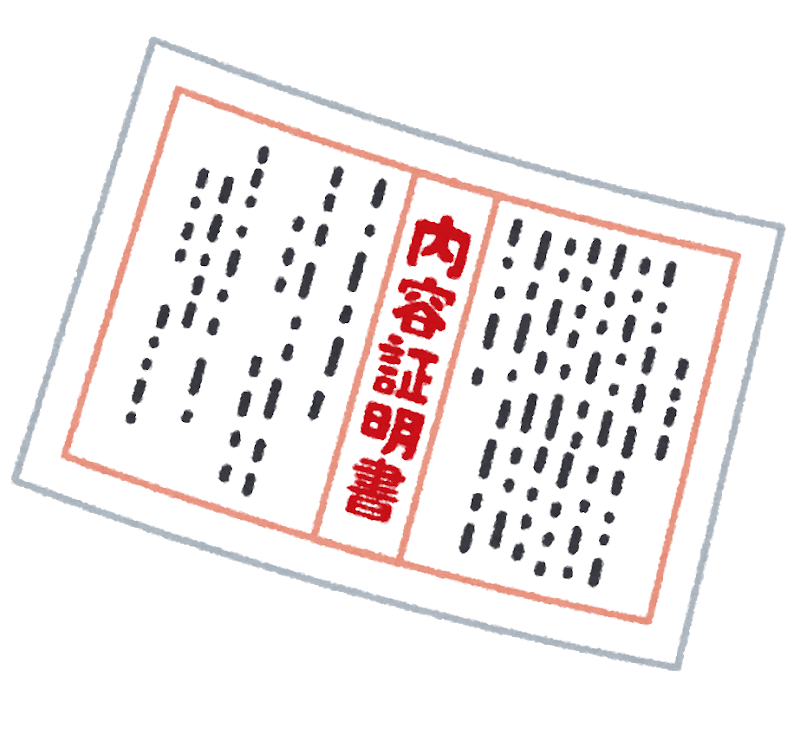
\includegraphics[width=\linewidth]{Figs/naiyo-shomei.png} 
\end{minipage}
\end{tabular}
\end{center}

※認証器で生成するユーザの鍵ペアを\alert{Credential Key Pair}、Attestされたその公開鍵証明書を\alert{Credential Certificate}と呼ぶ。
\end{frame}

\begin{frame}
\small 
Attestationの流れ。Attestationは2段階の証明で成立:
\begin{center}
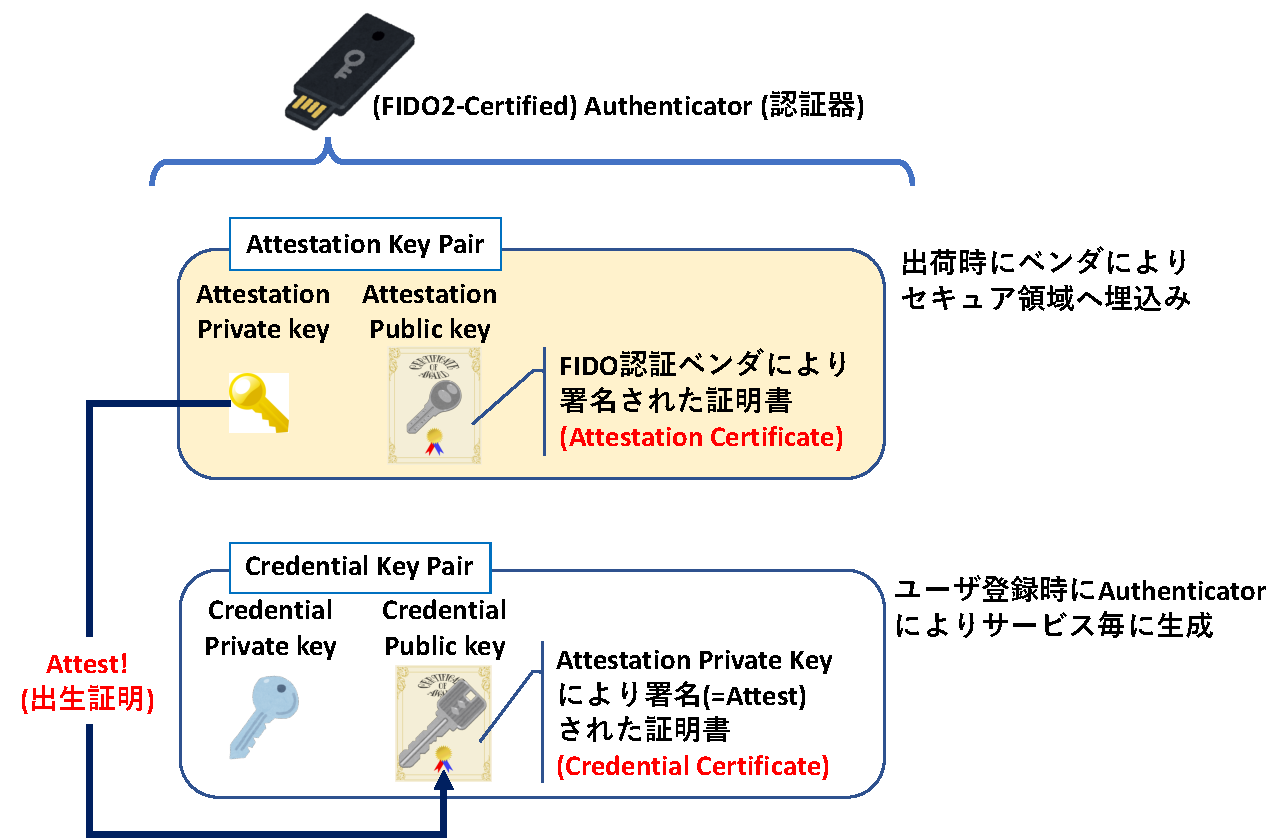
\includegraphics[width=0.7\linewidth]{Figs/webauthn-attestation.pdf}
\end{center}

ユーザ登録時にユーザ公開鍵(Credential Public Key)を出生証明して登録\\
$\Rightarrow$ Credential CertificateをAttestation Certificateで検証\\
$\Rightarrow$ Attestation CertificateをFIDO認証ベンダの公開鍵\footnote[frame]{\scriptsize ルート証明書}で検証
\end{frame}

\begin{frame}
\small
\begin{exampleblock}{\small 補足: Attestationの種類}
\footnotesize
\begin{itemize}
\setlength{\itemsep}{0ex}
 \item \textbf{Basic}: ベンダが認証器モデルごとに特有のAttestation Key Pairを埋込む。同じモデルの認証器では同じ鍵ペアでも良い。
 \item \textbf{Self}: Attestation Private Key = Credential Private Keyで、Credential Certificateが自己証明書になる。
 \item \textbf{AttCA}\footnote[frame]{\scriptsize Attestation Certificate Authority}: Attestation Certificateを動的に生成する手法。外部に信頼できる第三者の認証局を設け、認証器がAttestation (Identity) Key Pairを生成して、認証局へその公開鍵への署名を依頼。
 \item \textbf{ECDAA}\footnote[frame]{\scriptsize Elliptic Curve based Direct Anonymous Attestation; アルゴリズム仕様は現状ドラフト。}: 楕円曲線上の匿名認証 (Direct Anonymous Attestation; DAA) を利用して、認証器の情報を与えることなく出生証明を実現。
 \item \textbf{None}: Attestationなし。
\end{itemize}
\end{exampleblock}
\textbf{この資料ではBasic前提}。

BasicでもHW構造的に\alert{秘密鍵は認証器から取出せない}。
AttCAでは、認証器のTPMに埋め込まれた鍵を、証明書生成ではなく認証局との暗号通信用に用いる。
\end{frame}

\begin{frame}{WebAuthn ユーザ登録フロー}
以下のような流れでWebAuthnの認証のための登録を行う。
\begin{center}
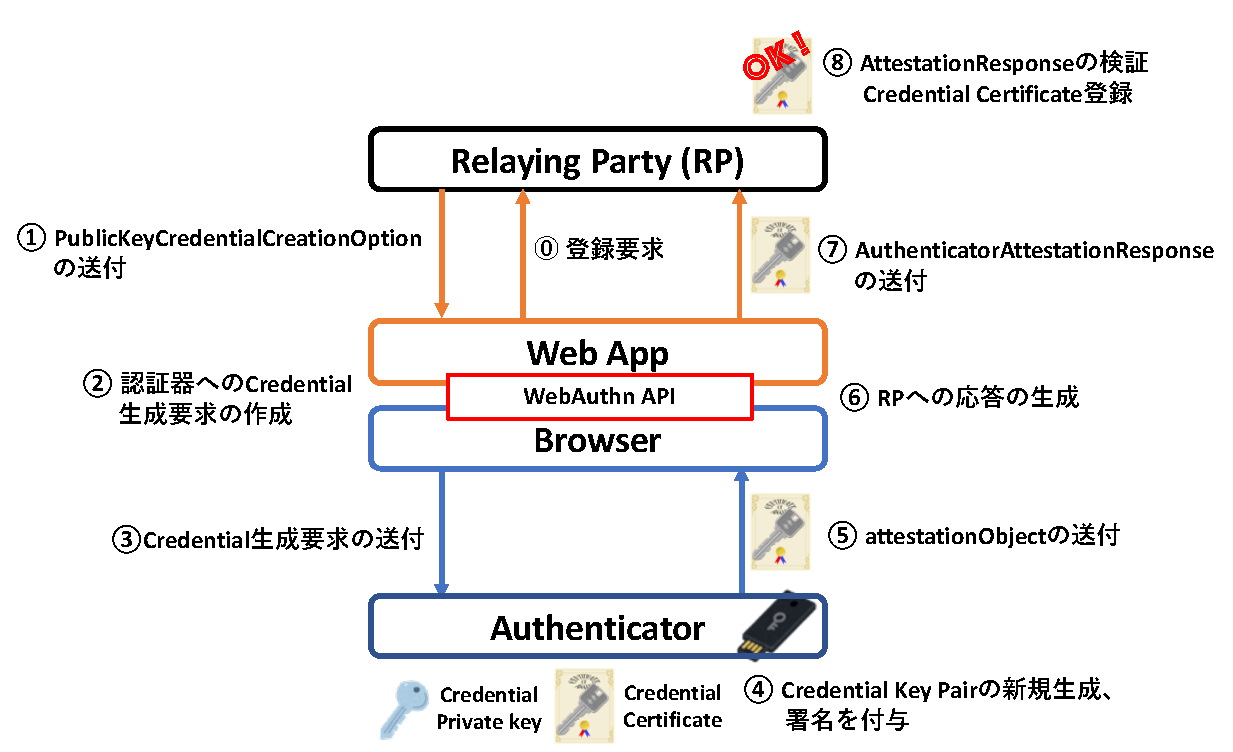
\includegraphics[width=0.8\linewidth]{Figs/webauthn-registration0.pdf}
\end{center}
単純に言うと、\textbf{Credential Certificateを生成、その出生証明を確認・登録}という処理。

\end{frame}

\begin{frame}
ここから、各ステップでやりとりされるデータを実際に確認していこう。
\end{frame}

\begin{frame}{WebAuthn ユーザ登録フロー: Credential生成要求}
a
\end{frame}

\begin{frame}{WebAuthn ユーザ登録フロー: Credential生成・取り出し}
a
\end{frame}

\begin{frame}{WebAuthn ユーザ登録フロー: Attestation!}
a
\end{frame}

\begin{frame}{WebAuthn ユーザ認証フロー}
WebAPIの観点では、認証器においてユーザ秘密鍵で署名生成。
\end{frame}

\section{まとめ}
\begin{frame}
\centering
{\huge まとめ}
\end{frame}

\begin{frame}
 
\end{frame}



% %%%%%%%%%%%%%%%%%%%%%%%%%%%%%%%%%%%%%%%%%%%%%%%%%%%%%%%%%%%%%%%%%%%%%%%%%%%%%%%%%%%%%%%%%%%%%%%%%%%
% \backupbegin

% \section{Backup}

% \begin{frame}
 
% \end{frame}

% \begin{frame}
% \frametitle{Appendix}
% This page is not counted.
% \end{frame}
% \backupend
\end{document}
%%%%%%%%%%%%%%%%%%%%%%%%%%%%%%%%%%%%%%%%%%%%%%%%%%%%%%%%%%%%%%%%%%%%%%%%%%%%%%%%%%%%%%%%%%%%%%%%%%%
%%%%%%%%%%%%%%%%%%%%%%%%%%%%%%%%%%%%%%%%%%%%%%%%%%%%%%%%%%%%%%%%%%%%%%%%%%%%%%%%%%%%%%%%%%%%%%%%%%%
%%%%%%%%%%%%%%%%%%%%%%%%%%%%%%%%%%%%%%%%%%%%%%%%%%%%%%%%%%%%%%%%%%%%%%%%%%%%%%%%%%%%%%%%%%%%%%%%%%%
%%%%%%%%%%%%%%%%%%%%%%%%%%%%%%%%%%%%%%%%%%%%%%%%%%%%%%%%%%%%%%%%%%%%%%%%%%%%%%%%%%%%%%%%%%%%%%%%%%%
%%%%%%%%%%%%%%%%%%%%%%%%%%%%%%%%%%%%%%%%%%%%%%%%%%%%%%%%%%%%%%%%%%%%%%%%%%%%%%%%%%%%%%%%%%%%%%%%%%%
%%%%%%%%%%%%%%%%%%%%%%%%%%%%%%%%%%%%%%%%%%%%%%%%%%%%%%%%%%%%%%%%%%%%%%%%%%%%%%%%%%%%%%%%%%%%%%%%%%%
